\documentclass{beamer}
\usetheme{metropolis}

\usepackage{changepage}
\usepackage{setspace}
\usepackage{amsmath,amssymb,amsthm}
\providecommand{\ol}{\overline}
\providecommand{\ul}{\underline}
\providecommand{\eps}{\varepsilon}
\providecommand{\half}{\frac{1}{2}}
\providecommand{\dang}{\measuredangle} %% Directed angle
\providecommand{\CC}{\mathbb C}
\providecommand{\FF}{\mathbb F}
\providecommand{\NN}{\mathbb N}
\providecommand{\QQ}{\mathbb Q}
\providecommand{\RR}{\mathbb R}
\providecommand{\ZZ}{\mathbb Z}
\providecommand{\dg}{^\circ}
\providecommand{\ii}{\item}
\providecommand{\setdiff}{\smallsetminus}
\providecommand{\alert}[1]{{\sffamily\textbf{\textcolor{blue}{#1}}}}
\providecommand{\inv}{^{-1}}
\providecommand{\mb}[1]{\mathbf{#1}}

\beamersetuncovermixins{\opaqueness<1>{25}}{\opaqueness<2->{15}}
\begin{document}
\title{Type Theory and Mathematical Logic}
\subtitle{PHI 108}
\author{Aditya Pahuja}
\date{October 29, 2024}

\begin{frame}
	\titlepage
\end{frame}

\begin{frame}\frametitle{Set theory}
	One modern foundational system of math is \emph{set theory},
	which defines all mathematical objects in terms of sets,
	which, informally, are collections of elements.
	For example, $\{1, 0, 8\}$ is a set whose elements are $1$, $0$, $8$.
	% TODO: \usepackage{graphicx} required
	\begin{figure}[h]
		\centering
		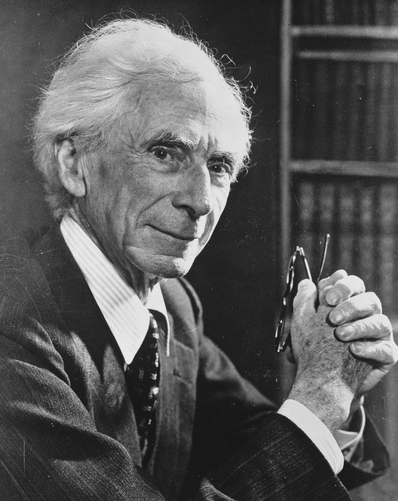
\includegraphics[width=0.3\linewidth]{russell}
		\caption{Bertrand Russell, a pioneer of mathematical logic.}
		\label{fig:russell}
	\end{figure}
\end{frame}

\begin{frame}\frametitle{Set theory notation}
	Two pieces of notation:
	\begin{itemize}
		\ii To describe a set, we use an expression like
		\[S = \{x : x\text{ has property $P$}\},\]
		which says ``$S$ is the set of elements $x$
		that have property $P$.'' For example
		\[\{x : x\text{ is a positive integer smaller than $3$}\}
		= \{1, 2\}.\]
		\ii If $S$ is a set, then we write $x\in S$ if $x$ is an element of $S$
		and $x\notin S$ if $x$ isn't an element of $S$.
		Thus $1\in\{1, 0, 8\}$ and $2\notin\{1, 0, 8\}$.
	\end{itemize}
\end{frame}

\begin{frame}\frametitle{Russell's paradox}
	\begin{itemize}
		\ii Early formulations of set theory
		(now called \emph{naive set theory})
		did not place any restrictions on the property $P$.
		\ii This led to \emph{Russell's paradox}, named after Bertrand Russell:
		consider the set
		\[R = \{S : S\notin S\}.\]
		\begin{itemize}
			\ii[$\circ$] On one hand, if $R\notin R$, then $R$ has
			the defining property of the set, so $R$ must be an element of $R$.
			\ii[$\circ$] On the other hand, if $R\in R$, then $R$
			does not have the defining property of the set,
			so $R$ cannot be an element of $R$.
		\end{itemize}
	\end{itemize}
\end{frame}

\begin{frame}\frametitle{The birth of type theory}
	Since the existence of $R$ led to a contradiction,
	mathematicians had two responses:
	\begin{itemize}
		\ii Some, like Ernst Zermelo, patched set theory
		to create modern set theory.
		\ii Russell created a version of what we now call \emph{type theory}.
	\end{itemize}
	
	\begin{adjustwidth}{15pt}{15pt}
		\begin{spacing}{0.8}
			\textit{\textcolor{gray}{\scriptsize
			Over time these solutions embedded themselves in academia and in
			culture, such that many of them them are now taken
			to be common sense. But what looks like common
			sense today was in the past not so common, and not
			seen as obviously sensible. More often than not,
			somebody somewhere had to struggle for it. (CPT 15)
			}}
		\end{spacing}
	\end{adjustwidth}
\end{frame}

\begin{frame}\frametitle{Basics of type theory: types}
	In type theory, every object has an inherent \emph{type}.
	\begin{itemize}
		\ii To declare that an object $x$ has a type $A$,
		we write $x : A$.
		\ii For example, we say that natural numbers
		have type $\NN$, so $x : \NN$ means that $x$ is a natural number.
	\end{itemize}
	The main idea is that objects are inseparable from their types:
	one cannot refer to an object without assigning it a type.
	
	\begin{adjustwidth}{15pt}{15pt}
		\begin{spacing}{0.8}
			\textit{\textcolor{gray}{\scriptsize
			But for the purpose of reasoning as clearly and as systematically as possible, it is important to use our words very carefully. This usually means avoiding metaphors, symbols, rhetorical questions, weasel words, euphemisms, tangents, equivocations, and
			`double speak'. When building a case for why something is true, or something else is not true, etc., it is important to say exactly what you mean, and eliminate ambiguities as much as possible. (CPT 80)
			}}
		\end{spacing}
	\end{adjustwidth}
	
\end{frame}

\begin{frame}\frametitle{Basics of type theory: functions}
	We can also talk about functions between types.
	Recall that a function $f$ with \emph{domain} $A$ and \emph{codomain} $B$
	is a rule for transforming elements of $A$ into elements of $B$.
	\begin{itemize}
		\ii We say that $f$ has type $A\to B$.
	\end{itemize}
\end{frame}

\begin{frame}\frametitle{Basics of type theory: more abstract types}
	To create new types, we must specify a few pieces of information:
	\begin{itemize}
		\ii A \emph{formation} rule, which describes
		the constituents of the new type.
		\ii An \emph{introduction} rule, which describes
		how to construct objects of the new type.
		\ii An \emph{elimination} rule, which defines
		functions that help extract information about objects of the type.
		\ii A \emph{computation} rule, which describes
		what the functions from the elimination rule output.
		\ii Optionally, a \emph{uniqueness} rule,
		which essentially says that objects of a type are uniquely determined by
		the results of elimination rules applied to it.
	\end{itemize}
\end{frame}

\begin{frame}\frametitle{The punchline}
	The kicker is that type theory can function as a system of logic
	with the main principle that \emph{every proposition is a type}.
	\begin{adjustwidth}{15pt}{15pt}
		\begin{spacing}{0.8}
			\textit{\textcolor{gray}{\scriptsize By following the guidelines noted above \dots, we can craft the kinds of sentences that can be used to build arguments. Such sentences are called propositions; or they are also sometimes called statements and claims. A proposition is a simple sentence that has just one meaning, for it expresses one thought according to the rules of grammar in the language in which it is expressed. (CPT 82)}}
		\end{spacing}
	\end{adjustwidth}
\end{frame}

\begin{frame}\frametitle{How do we represent truth?}
	\begin{itemize}
		\ii A proposition is true if we can construct
		an object of the corresponding type.
		\ii Implication corresponds naturally to functions!
	\end{itemize}
	
	\begin{adjustwidth}{15pt}{15pt}
		\begin{spacing}{0.8}
			\textit{\textcolor{gray}{\scriptsize
			What is truth? The origin of the English word truth is in Anglo-Saxon words like getriewe, treow, and troth, words relating to faithfulness, fidelity, honesty, promise keeping, and loyalty, especially in relation to an important undertaking. Truth, in the kind of logic we’ve been discussing here, is a property of propositions. (CPT 84)
			}}
		\end{spacing}
	\end{adjustwidth}
\end{frame}

\begin{frame}\frametitle{Logical connectives: Conjunction}
	\begin{itemize}
		\ii Formation: Given propositions $P$ and $Q$,
		we form the type $P\land Q$.
		\ii Introduction: Given $p_1 : P$ and $q_1 : Q$,
		we can construct an object $(p_1, q_1) : P\land Q$.
		\ii Elimination: Given $(p_1, q_1):P\land Q$, we have functions
		$L(p_1, q_1) : P$
		and $R(p_1, q_1) : Q$.
		\ii Computation: $L(p_1, q_1) = p_1 : P$
		and $R(p_1, q_1) = q_1 : Q$.
		\ii Uniqueness: Given $z : P\land Q$,
		$z = (L(z), R(z))$.
	\end{itemize}

	Disjunctions are significantly more complicated
	and will be left as reading for the interested viewer.
\end{frame}

\begin{frame}\frametitle{Logical connectives: Equivalence}
	\begin{itemize}
		\ii Formation: Given propositions $P\to Q$ and $Q\to P$,
		we form the type $P\iff Q$.
		\ii Introduction: Given $f_1 : P\to Q$
		and $f_2 : Q\to P$, we can produce an object $(f_1, f_2) : P\iff Q$.
		\ii Elimination: Given $(f_1, f_2):P\iff Q$, we have functions
		$L(f_1, f_2) : P\to Q$
		and $R(f_1, f_2) : Q\to P$.
		\ii Computation: $L(f_1, f_2) = f_1 : P\to Q$
		and $R(f_1, f_2) = f_2 : Q\to P$.
		\ii Uniqueness: Given $z : P\iff Q$,
		$f = (L(f), R(f))$.
	\end{itemize}
\end{frame}

\begin{frame}\frametitle{Logical connectives: Negation}
	To talk about falseness, we could describe a construction of
	$\neg P$ given $P$, but there is a subtle trick to avoid this!
	\begin{itemize}
		\ii We define a type False with no objects (thus it is not true).
		False only has a (trivial) formation rule and an elimination rule
		that essentially produces an object of any type.
		\ii We think of $\neg P$ as shorthand
		for the type $P\to\operatorname{False}$ since, if $P$ is true,
		then we can find an object of type False,
		which means that $P$ cannot be true.
	\end{itemize}
\end{frame}

\begin{frame}\frametitle{An example}
	Modus tollens says that if $P\to Q$ and $\neg Q$, then $\neg P$.
	In type theory, this means we have to construct an object of type
	$\neg P$ given objects of type $P\to Q$ and $\neg Q$.
	\begin{itemize}
		\ii Let $f_1 : P\to Q$ and $f_2 : Q\to\operatorname{False}$,
		recalling that $\neg Q$ is shorthand for $Q\to\operatorname{False}$.
		The composed function $f_2\circ f_1$
		is then a function $P\to\operatorname{False}$, so
		$f_2\circ f_1 : \neg P$.
	\end{itemize}
	
	A fun exercise: prove that $P\land Q\iff Q\land P$.

	\begin{adjustwidth}{15pt}{15pt}
		\begin{spacing}{0.8}
			\textit{\textcolor{gray}{\scriptsize
			The validity of an argument is determined not by what it says, but by its form. This means that when we assess the validity of an argument, we assume that the premises are true. \dots When we test for an argument’s validity, we ignore all questions about whether the propositions are true or false. Instead, we only look at the way the propositions are arranged in relation to each other, and whether they conform to a correct logical structure. (CPT 95)
			}}
		\end{spacing}
	\end{adjustwidth}
\end{frame}

\begin{frame}\frametitle{Computer science}
	Many modern programming languages are \emph{typed},
	meaning all variables and functions have to have a type!
	\begin{figure}
		\centering
		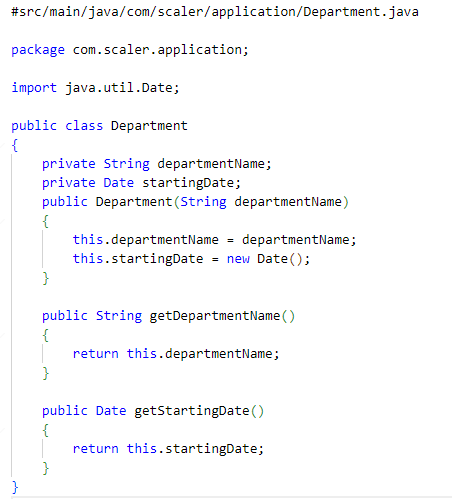
\includegraphics[scale=0.25]{javacode.png}
		\caption{Some code in Java.}
	\end{figure}
\end{frame}

\begin{frame}\frametitle{Proof assistants}
	Proof assistants are software tools that aid in the creation of
	completely rigorous mathematical proofs.
	Some, like Lean 4, implement a version of type theory
	called \emph{dependent type theory}.
	
	\begin{figure}[h]
		\centering
		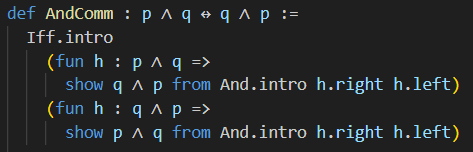
\includegraphics[width=0.7\linewidth]{andcommpf}
		\caption{A proof that $P\land Q\iff Q\land P$ in Lean 4.}
		\label{fig:andcommpf}
	\end{figure}
	
\end{frame}

\begin{frame}\frametitle{Linguistics}
	Type theory can be used to represent semantic structures in linguistics.
	One way to do this:
	\begin{itemize}
		\ii $e$ and $t$ are basic types for individuals and truth values.
		\ii If $a$ and $b$ are types then so is $\langle a,b\rangle$,
		which is the type of functions from entities of type $a$
		to entities of type $b$.
		\ii For example, in the sentence ``Bill is blond,''
		``Bill'' has type $e$ and ``blond'' has type $\langle e,t\rangle$
		(and the sentence has type $t$).
	\end{itemize}
\end{frame}

\begin{frame}\frametitle{Further questions}
	\begin{itemize}
		\ii Why is mathematical formalism important?
		\ii Are there paradoxes in versions of type theory
		similar to Russell's paradox in (naive) set theory?
		\ii How does type theory relate to other foundational systems
		of math and logic?
	\end{itemize}
\end{frame}

\begin{frame}\frametitle{Additional reading}
	Links!
	\begin{itemize}
		\ii\textcolor{blue} {\href{https://ncatlab.org/nlab/show/propositional+logic+as+a+dependent+type+theory}{Propositional logic as a dependent type theory}}
		\ii\textcolor{blue} {\href{https://leanprover.github.io/theorem_proving_in_lean4/propositions_and_proofs.html}{Theorem Proving in Lean 4}}
		\ii\textcolor{blue} {\href{https://www.coli.uni-saarland.de/courses/semantics-06/lectures/lect2.pdf}{Type theory in linguistics}}
	\end{itemize}
\end{frame}

\end{document}

